\documentclass[11pt]{beamer}
\usepackage{helvet} %font
\beamertemplatenavigationsymbolsempty
\usetheme{JuanLesPins}
\usefonttheme{structurebold}

\usepackage[french]{babel}
\usepackage[utf8]{inputenc}
\usepackage[T1]{fontenc}
\usepackage{amssymb,amsmath}
\usepackage{tikz}
\usepackage{geometry}
\usepackage{xcolor,colortbl}
\usetikzlibrary{arrows,positioning}
\usepackage{listings}

\AtBeginSubsection[]
{
   \begin{frame}
	\small \tableofcontents[currentsection]
   \end{frame}
}

\newenvironment{slide}[1]{%
\begin{frame}[environment=slide]
\frametitle{#1}
}{%
\end{frame}
}
\setbeamercolor{structure}{fg=red}
\setbeamercolor{frametitle}{bg=black,fg=white}
\definecolor{gris}{gray}{0.6}
\definecolor{grisclair}{gray}{0.9}

\newtheorem{exercice}{Exercice}


\newcommand{\Python}[1]{
	{\small	\lstinputlisting[language=Python]{./#1.py}}
}
\newenvironment{pyenvsmall}
	{ \ttfamily \tiny }
	{\par  }

\newcommand{\Pythonsmall}[1]{
	{\scriptsize \lstinputlisting[language=Python]{./#1.py}}
}

\title{Machine Learning X : Dimension}
\author{Nicolas Bourgeois}
\date{}
\begin{document}

\section{Principe}
\subsection{Pulvérisation}
\begin{frame}{Décomposition du risque}
$$D(\tilde{F}) - ROPT = D(\tilde{F}) - \min_{\tilde{g}\in Z}\mathbb{E}(LF(\tilde{g}(X),Y))$$
$$+\min_{\tilde{g}\in Z}\mathbb{E}(LF(\tilde{g}(X),Y)) - ROPT $$
\\ \vspace{0.3cm}
Comment optimiser $Z$ ?
\end{frame}

\begin{frame}{Pulvérisation}
Un ensemble $X \subset E$ est dit pulvérisé par une famille de sous-ensembles $H=(H_i \subset E)$ si :\\

$$H \cap X \supset 2^X$$

Autrement dit, si tout sous-ensemble de $X$ peut être associé à un élément de $H$. 

\end{frame}

\begin{frame}{Exemple}

Si $X$ est formé de 3 points non alignés du plan $E$, il est pulvérisé par $H$ l'ensemble des demi-plans.


\end{frame}

\begin{frame}{Exemple}
\begin{figure}
\begin{tikzpicture}
\node[fill=blue] at (0,0) (1){};
\node[fill=red] at (1,2) (2){};
\node[fill=red] at (2.5,1) (3){};
\end{tikzpicture}
\end{figure}
\end{frame}
\begin{frame}{Exemple}
\begin{figure}
\begin{tikzpicture}
\node[fill=red] at (0,0) (1){};
\node[fill=red] at (1,2) (2){};
\node[fill=red] at (2.5,1) (3){};
\end{tikzpicture}
\end{figure}
\end{frame}

\begin{frame}{exercice}

\begin{exercice}
Comment peut-on pulvériser un ensemble de trois points alignés ?
\end{exercice}
\begin{exercice}
Comment peut-on pulvériser un ensemble de quatre points situés aux sommets d'un carré ?
\end{exercice}

\end{frame}

\begin{frame}{Exemple}
\begin{figure}
\begin{tikzpicture}
\node[fill=blue] at (0,0) (1){};
\node[fill=red] at (1,1) (2){};
\node[fill=blue] at (2,2) (3){};
\end{tikzpicture}
\end{figure}
\end{frame}

\begin{frame}{Exemple}
\begin{figure}
\begin{tikzpicture}
\node[fill=blue] at (0,1) (1){};
\node[fill=red] at (-1,0) (2){};
\node[fill=blue] at (0,-1) (3){};
\node[fill=red] at (1,0) (2){};
\end{tikzpicture}
\end{figure}
\end{frame}


\begin{frame}{Pulvérisation par une famille d'estimateurs}
Un ensemble $X \subset E$ est dit pulvérisé par une famille d'estimateurs $F=(f_i \in G^E)$ si il est pulvérisé par ses images réciproques $(f^{-1}_i(y))$\\

\vspace{0.2cm}

Autrement dit, si tout sous-ensemble de $X$ peut être discriminé par un élément de $F$. 

\end{frame}

\begin{frame}{Perceptron}

Le perceptron (mono-couche) à $n$ entrées de coefficients $w$ et de seuil $\theta$ est défini par :

$$ f: E=\mathbb{R}^p \longrightarrow \{0,1\}$$
$$ f(x)=1 \Leftrightarrow w\cdot x > \theta$$ 

\end{frame}

\begin{frame}{Exercice}

\begin{exercice}
Géométriquement, à quoi correspond un perceptron ? Combien de points non coplanaires est-il capable de pulvériser pour un $p$ donné ?
\end{exercice}

\end{frame}

\subsection{dimension de Vapnik–Chervonenkis}

\begin{frame}{dimension de Vapnik–Chervonenkis}
$$VC(H) = \max \{i\in \mathbb{N}, \exists X, |X|=i \vee H \cap X \supset 2^X \}$$
\\ \vspace{0.2cm}

Pour une famille d'estimateurs, la dimension de Vapnik–Chervonenkis correspond à la taille \textbf{maximale} d'un ensemble que cette famille peut pulvériser.

\end{frame}

\begin{frame}{}
$$D(\tilde{F}) - ROPT = D(\tilde{F}) - \min_{\tilde{g}\in Z}\mathbb{E}(LF(\tilde{g}(X),Y))$$
$$+\min_{\tilde{g}\in Z}\mathbb{E}(LF(\tilde{g}(X),Y)) - ROPT $$
\\ \vspace{0.3cm}
Comment optimiser $Z$ ?
\end{frame}

\begin{frame}{dimension et convergence (1)}

Si $VC(Z)$ est bornée, $$D(\tilde{F}) - \min_{\tilde{g}\in Z} \mathbb{E}(LF(\tilde{g}(X),Y))\longrightarrow 0$$\\

\pause
\vspace{0.2cm}

Si $VC(Z)$ n'est pas bornée, $$\min_{\tilde{g}\in Z}\mathbb{E}(LF(\tilde{g}(X),Y))- ROPT$$ est potentiellement meilleure.

\end{frame}

\begin{frame}{dimension et convergence (1)}
Si les $(X_i,Y_i) $ sont iid et

$$ n = \Theta\left(\frac{VC(Z)-\log(\delta)}{\epsilon^2}\right)$$

Alors :

$$ \mathbb{P}\left(D(\tilde{F}) - \min_{\tilde{g}\in Z}\mathbb{E}(LF(\tilde{g}(X),Y))<\epsilon\right) >1-\delta$$
\end{frame}

\begin{frame}{Une situation idéale}
On peut trouver des familles croissantes d'estimateurs $Z_k$ tels que :
$$(X_i,Y_i)_{i\leq n},n\rightarrow \infty $$
$$k \longrightarrow \infty$$
$$VC(Z_k) \rightarrow \infty$$
$$VC(Z_k)\frac{\log n}{n} \longrightarrow 0$$
ET\\

\vspace{0.2cm}
$$\min_{\tilde{g}\in Z_k}\mathbb{E}(LF(\tilde{g}(X),Y))- ROPT \longrightarrow 0$$

\end{frame}

\section{SVM}

\subsection{SVM linéaire}

\begin{frame}{Cas binaire}
$$G=\{-1,1\}$$
$$LF = \textbf{1}_{Y\neq Y'}$$
$$Z = \{x\mapsto a+b\cdot x,(a,b)\in E\}$$

Un ensemble est séparable si :
$$\exists g \in Z,\forall i, g(X_i)>0 \Leftrightarrow Y_i=1$$

\end{frame}

\begin{frame}{Marge optimale}
On veut optimiser :
$$\max_{a,b}\min_{i} d(X_i,\Delta_g)$$
$$= \max_{a,b}\min_{i} \frac{a+b\cdot X_i}{|b|}$$
$$= \min_{\forall i, (a+b\cdot X_i)Y_i \geq 1} |b|^2$$
\end{frame}

\begin{frame}
\begin{exercice}
Retrouvez graphiquement ces formules
\end{exercice}
\end{frame}

\begin{frame}
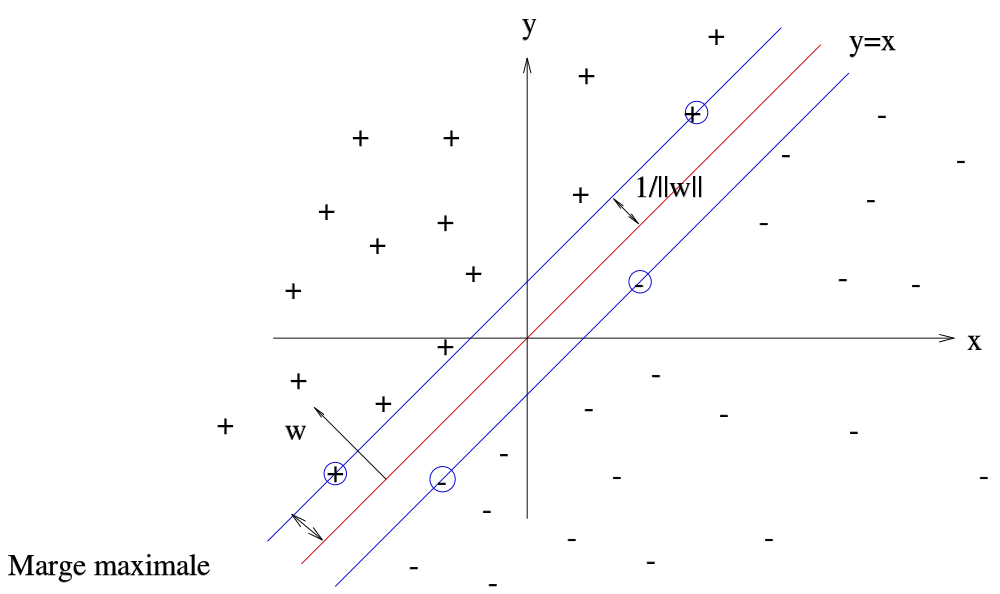
\includegraphics[scale=0.3]{svm}
\end{frame}

\begin{frame}{Cas non séparable}
On veut optimiser :
$$\min_{\forall i, (a+b\cdot X_i)Y_i \geq 1-c_i} |b|^2+p\sum c_i$$
\end{frame}

\begin{frame}
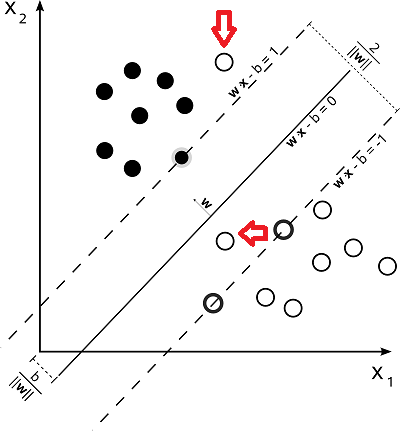
\includegraphics[scale=0.6]{relax}
\end{frame}

\begin{frame}
On se ramène donc à un problème d'optimisation classique:\\ \vspace{0.3cm}
\begin{itemize}
	\item méthodes quadratiques,
	\item méthodes de gradient,
	\item complexité dépendante de la pénalisation
\end{itemize}
\end{frame}

\begin{frame}
\begin{exercice}
A partir des données iris, en vous restreignant aux largeurs/longueurs de sépales et aux deux premières classes, écrivez un programme qui en fonction d'une pénalité $p$ trouve la séparation optimale. Affichez la droite de séparation pour chaque pénalité.
\end{exercice}
\end{frame}

\begin{frame}{résultat}
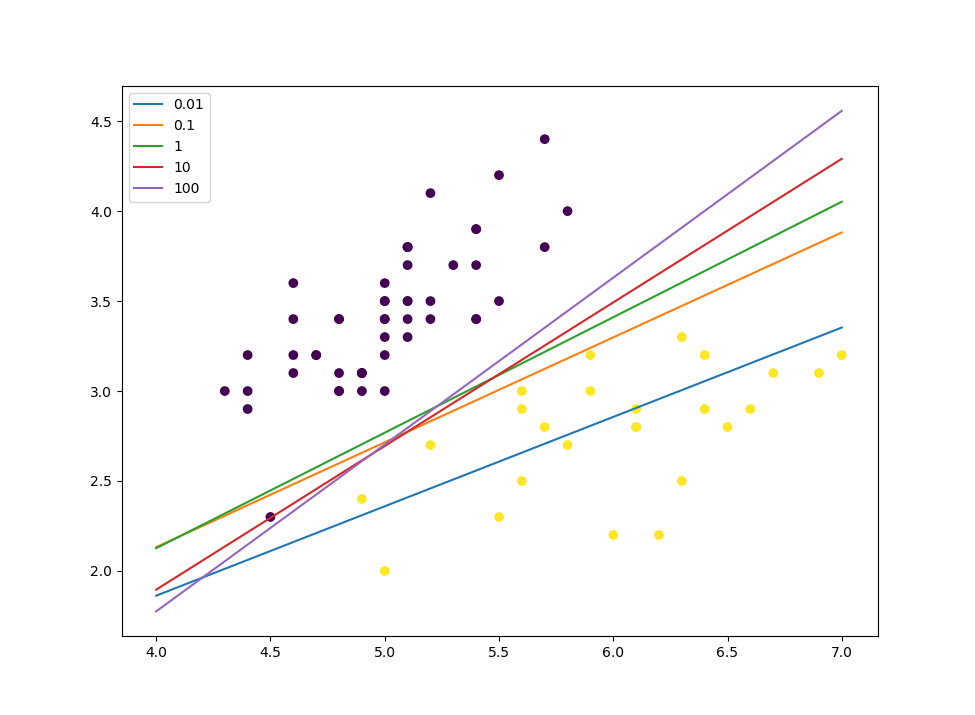
\includegraphics[scale=0.4]{ext12}
\end{frame}

\begin{frame}{solution}
\Pythonsmall{ext12}
\end{frame}

\subsection{SVM à kernel}

\begin{frame}{Séparabilité et dimension}
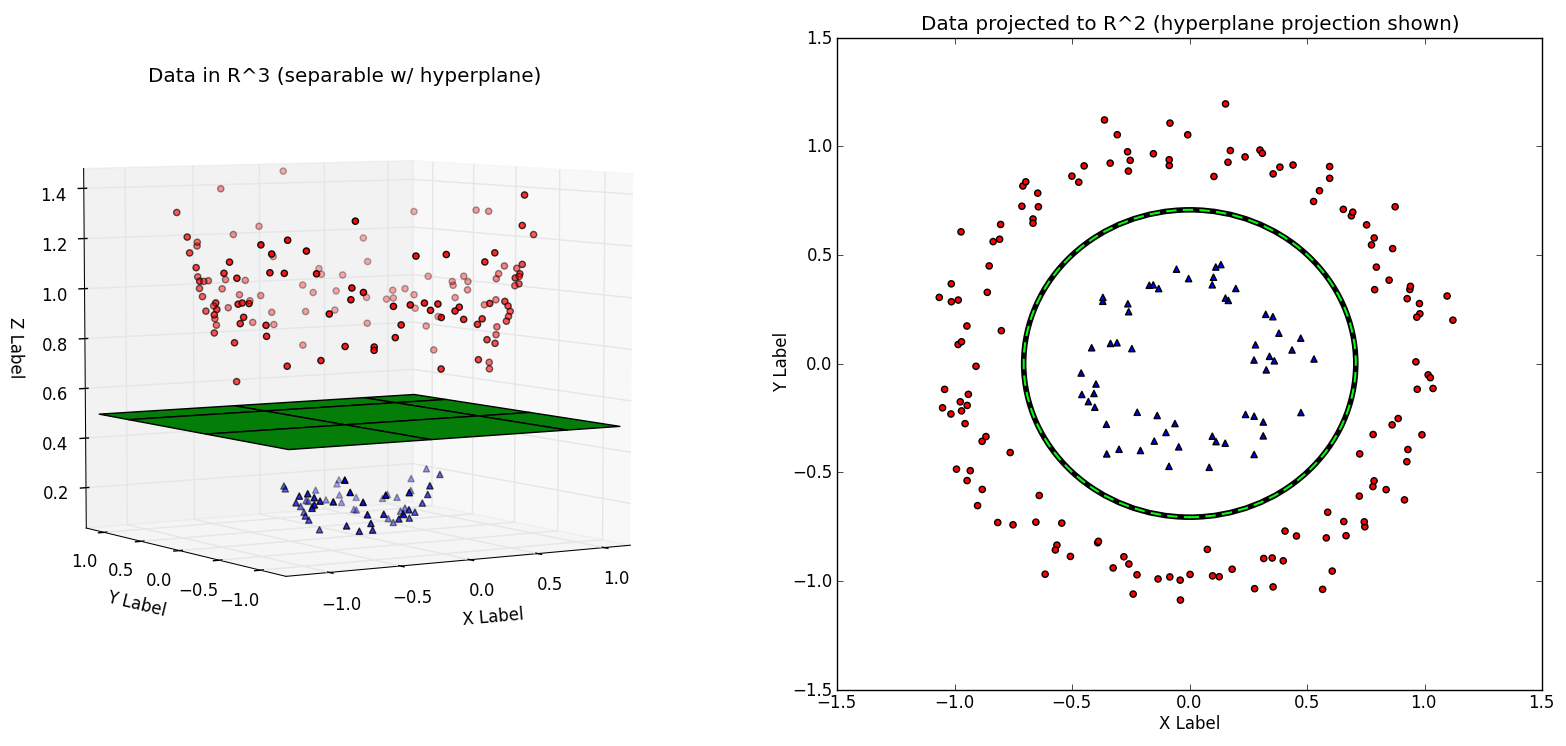
\includegraphics[scale=0.25]{kernel}
\end{frame}

\begin{frame}{Séparabilité et dimension}

Comme pour la pulvérisation, l'espérance du nombre de points séparables vérifie $n \sim 2p$ où $p$ est la dimension de $E$.\\

\pause
\vspace{0.2cm}

On considère $ \Phi : E \rightarrow E'$ où $dim(E')>dim(E)$.

\pause
\vspace{0.2cm}

Et le problème devient 
$$\min_{\forall i, (a+b\cdot \Phi(X_i))Y_i \geq 1-c_i} |b|^2+p\sum c_i$$

\end{frame}

\begin{frame}{Problème Dual}

Problème primal :

$$\min_{\forall i, (a+b\cdot \Phi(X_i))Y_i \geq 1-c_i} |b|^2+p\sum c_i$$

Problème dual  :

$$\max_{\sum a_iY_i=0,\forall i, 0\leq a_i \leq p} 2\sum a_i-\sum\sum a_ia_jY_iY_j\Phi(X_i)\cdot\Phi(X_j)$$


\end{frame}

\begin{frame}{Problème avec Kernel}

Problème primal :

$$\min_{\forall i, (a+b\cdot \Phi(X_i))Y_i \geq 1-c_i} |b|^2+p\sum c_i$$

Problème kernelisé  :

$$\max_{\sum a_iY_i=0,\forall i, 0\leq a_i \leq p} 2\sum a_i-\sum\sum a_ia_jY_iY_jk(X_i,X_j)$$


\end{frame}

\end{document}